\documentclass[11pt,a4paper]{report}
\usepackage{amsmath}
\usepackage{booktabs}
\usepackage{graphics}
\usepackage[dvipdfmx]{graphicx}
\usepackage{epsfig}
\DeclareGraphicsExtensions{.eps,.pdf,.jpg,.png}
\DeclareGraphicsRule{.jpg}{eps}{.bb}{}
\everymath{\displaystyle}
\setlength\parindent{0pt}
\begin{document}

\title{Project2 Report}

\author{Ye Feiyang \and Li Jianliang \and Yuan Xiaojie}

\date{July 25, 2012}

\maketitle

\section*{Introduction}
In the MAC sublayer, Random Access Control is a very important part. There are four kinds of Random Access Control protocols: pure ALOHA, slotted ALOHA, CSMA and CSMA/CD. This project will simulate these four protocols to see their transmission efficiency and compare their performance. By doing this, it can be determined which protocol is suitable for a certain situation and helps us to understand how each protocol works.

\section*{Pure ALOHA}
\subsection*{Theories}
ALOHA was devised by Norman Abramson in the 1970s to solve the channel allocation problem. The basic idea of pure ALOHA is that users(or stations) can transimit frames whenever they have, which is totally random. Of course, when different users are transmiting their frames at the same time, those frames will collide and all of them will be damaged. A sender can find out whether its transmission succeed by checking the acknowledgements from the receiver. If the frame was damadged, it waits for a random time and send again. \\

Given the following parameters: \\

\qquad	\(X\): frame transmission time \\

\qquad	\(N\): average \# of frames genereted per frame time \\

\qquad	\(G\): load, average \# of transmission attempts per frame time \\

\qquad	\(k\): \# of transmissions attempts per frame time \\

\qquad	\(P\): probablity of a successful frame transmission \\

\qquad	\(S\): throughput, average \# of successful frames per frame time \\

We can derive that the probability that \(k\) frames are generated during a frame time \(X\) is given by the Poisson distribution \\

\qquad	\(P(k) = \frac{G^ke^{-G}}{k!}\) \\

So the probability of zero frames during the \(2G\) vulnerable time is \\

\qquad \(P(0)|_{G=2G} = e^{-2G}\) \\

Then the throughput is given by \\

\qquad \(S = Ge^{-2G}\) \\

for which the maximum occurs at \(G = 0.5\) with \(S = 1/2e \approx 0.184\) and the \(S - G\) graph is shown on "Figure 1".

\subsection*{Assumptions}

1. The length of each frame remains the same. \\
2. There is no propagation delay which means that one user can know whether its frames transmission succeed as soon as it finished its transimission. \\
3. The probability of an arrival during a short time interval \(\Delta t\) is propotional to the length of interval, and does not depend on the origin of the interval. \\
4. The probability of having multiple(\(>\) 1) arrivals during a short time interval \(\Delta t\) approaches 0;

\subsection*{Simulation}
In the simulation program, an two-dimensional array containing 0s and 1s is used to represent states of different users at each short time interval \(\Delta t\). For example, statest[\emph{userNum}][\emph{simulateTime}] is an \emph{userNum}\(\times\)\emph{simulateTime} array, its Nth(0 \(<\) N \(<\) \emph{userNum}) row represents that the Nth user's states from 0th to (\emph{simulateTime}-1)th short time interval. "0" is used when the user is not transmitting data at a certain short time interval and "1" is used otherwise. \\

The array can be expressed graphically like this: \\

states[\emph{N}][\emph{M}]: \\

\qquad user1: 111100111101111\(\cdots\)0111100000011110000000 \\

\qquad user2: 000011110000000\(\cdots\)00011110000000001111 \\

\qquad\quad \(\vdots\) \hspace{35mm} \(\vdots\) \\

\qquad userN: \hspace{-0.5mm}\(\underbrace{000000000111100\cdots1111000111100011110000}_\text{M short time intervals}\) \\

Since the frame length(frameLen) is assumed to be constant, the number of consetutive 1s remains the same(except the frames at the end of each row). The above example always has 4 consetutive 1s which represents a 6-slot length frame. \\

At the beginnig of each simulation, the array need to be initialized based on a given probability \(p\) which is the probability that a user generates a frame during a certain short time interval \(\Delta t\). Once the first state is initialized to be 1, its consetutive (frameLen - 1) states should all be set to 1. This initialization process is conducted by the function \emph{generate\_frame()}.\\

Then at each short time interval, the states of each user are checked and using function \emph{check\_collision}, three status(\emph{COLLISION}, \emph{NO\_COLLISION} and \emph{IDLE}) are marked. \\

If a collision is detected for a user, it pushs all its 1s and 0s backwards for a random time using function \emph{wait\_for\_random\_time()}. To be noticed, the random time should be between 0 and the maximum simulate time and it is set to \emph{SIMULATE\_TIME}/2 in the codes. \\

Finally, the driven function \emph{pure\_aloha\_simulate()} is called in \(main()\) to simulate and output the throughput \emph{S}.


\subsection*{Results}
Several global parameters are set as below: \\
\emph{USER\_NUM = 10} \\
\emph{SIMULATE\_TIME = 1000} \\
\emph{FRAME\_LEN = 4} \\

Then the propability \emph{p} are set differently to archive various \emph{G}, and for each \emph{G}, the simulation is run 1000 times to get an average \emph{S}. The data are recorded in the following table and the figure is shown on "Figure 1". \\
\begin{table}[htbp]
\begin{tabular}{lcccccccccc}
\toprule
p & 0 & 0.01 & 0.02  & 0.03 & 0.04 & 0.05 & 0.10 & 0.15 & 0.20 & 0.30 \\
\midrule
Num & 0 & 45 & 52 & 52 & 53 & 56 & 61 & 67 & 66 & 74 \\
\bottomrule
\end{tabular}
\end{table}

\begin{figure}
\centering
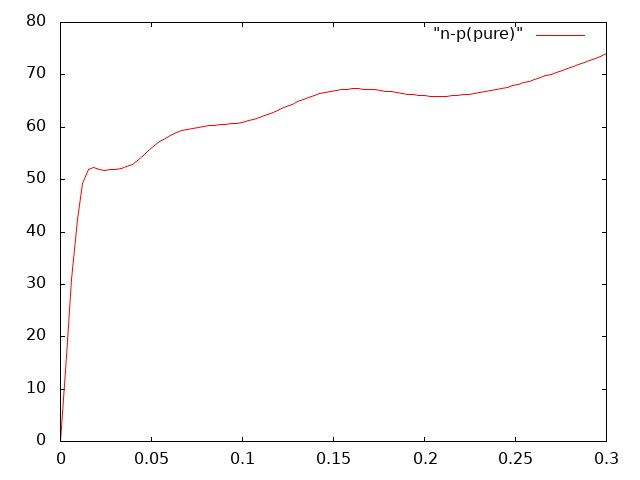
\includegraphics[width=0.5\textwidth]{1_1.jpg}
\caption{n-p Graph for Pure ALOHA}
\end{figure}

The number of attempts per frame time \(G\) is calculated as \(G = p*USER\_NUM\) and throughput \(S\) is calculated as \(S = successNum/250\). The data are recorded in the following table and the figure is shown on "Figure 2".
\begin{table}[htbp]
\begin{tabular}{lcccccccccc}
\toprule
G & 0 & 0.1 & 0.2  & 0.3 & 0.4 & 0.5 & 1.0 & 1.5 & 2.0 & 3.0 \\
\midrule
S & 0 & 0.183 & 0.209 & 0.211 & 0.215 & 0.224 & 0.247 & 0.269 & 0.268 & 0.300 \\
\bottomrule
\end{tabular}
\end{table}

\begin{figure}
\centering
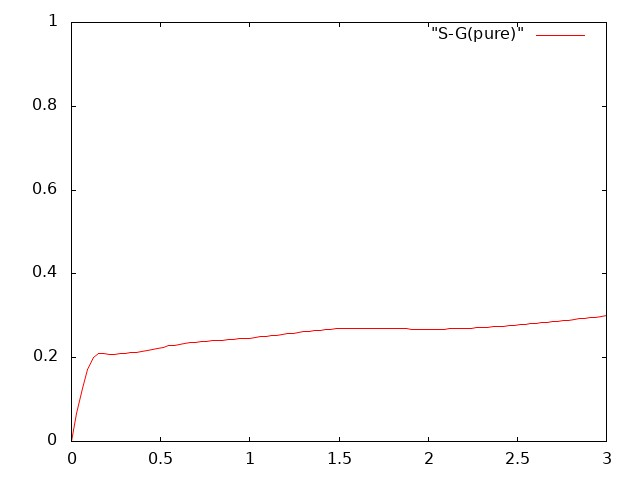
\includegraphics[width=0.6\textwidth]{1_2.jpg}
\caption{S-G Graph for Pure ALOHA}
\end{figure}

\subsection*{Analysis}
From the data above, the maximum value of \(S\) is approximately    when \(G\) is . Unfortunately, the result doesn't match well with the theory with \(S_{max} = 0.184\) at \(G = 0.5\). This may come from some inevitable drawbacks of the simulation model. \\

For example, the maximum random wait time is set to be \emph{SIMULATE\_TIME/2} and this may be a too long time so that when many users wait out of the simulate bound, the remaining users can almost send all of their frames. \\


\section*{Slotted ALOHA}
\subsection*{Theories}
Slotted ALOHA is an advanced version of pure ALOHA. It divides time into descrete slots that each frame can only be sent at the beginning of each time slot. Moreover, slotted ALOHA requires global time synchronization so that the same slot boundaries can be agreed by all the users. \\

The vulnerable time for slotted ALOHA is half of the one for pure ALOHA. So the probability of zero frames during the G vulnerable time is \\

\qquad \(P(0)|_{G=G} = e^{-G}\) \\

Then the throughput is given by \\

\qquad \(S = Ge^{-G}\) \\

for which the maximum occurs at \(G = 1\) with \(S = 1/e \approx 0.368\) and the \(S - G\) graph is shown on "Figure 1".

\subsection*{Assumptions}
1. Each frame can only be sent at the beginning of each time slot. \\
2. All of the rest are same as pure ALOHA.

\subsection*{Simulation}
Compared to pure ALOHA, the only difference for slotted ALOHA is that frames are only generated at the beginning of a time slot. \\

For example, the frames for userK can be only like the following format(the length of a time slot is 4 which is the same as the frame length): \\

\qquad userK: 1111 0000 1111 1111 1111 0000 \(\cdots\) 1111 0000 1111 1111 \\

\subsection*{Results}
Table for \(p\) and \(successNum\) is shown below and \(n-p\) graph is shown on "Figure 3".
\begin{table}[htbp]
\begin{tabular}{lcccccccccc}
\toprule
p & 0 & 0.01 & 0.02  & 0.03 & 0.04 & 0.05 & 0.10 & 0.15 & 0.20 & 0.30 \\
\midrule
Num & 0 & 65 & 85 & 94 & 97 & 92 & 80 & 73 & 69 & 65 \\
\bottomrule
\end{tabular}
\end{table}

\begin{figure}
\centering
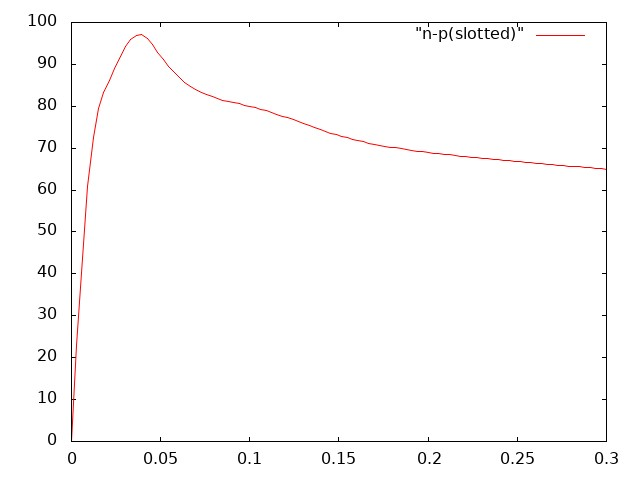
\includegraphics[width=0.5\textwidth]{2_1.jpg}
\caption{n-p Graph for Slotted ALOHA}
\end{figure}

Table for \(G\) and \(S\) is shown below and \(S-G\) graph is shown on "Figure 4".
\begin{table}[htbp]
\begin{tabular}{lcccccccccc}
\toprule
G & 0 & 0.1 & 0.2  & 0.3 & 0.4 & 0.5 & 1.0 & 1.5 & 2.0 & 3.0 \\
\midrule
S & 0 & 0.262 & 0.341 & 0.377 & 0.391 & 0.369 & 0.323 & 0.292 & 0.280 & 0.263 \\
\bottomrule
\end{tabular}
\end{table}

\begin{figure}
\centering
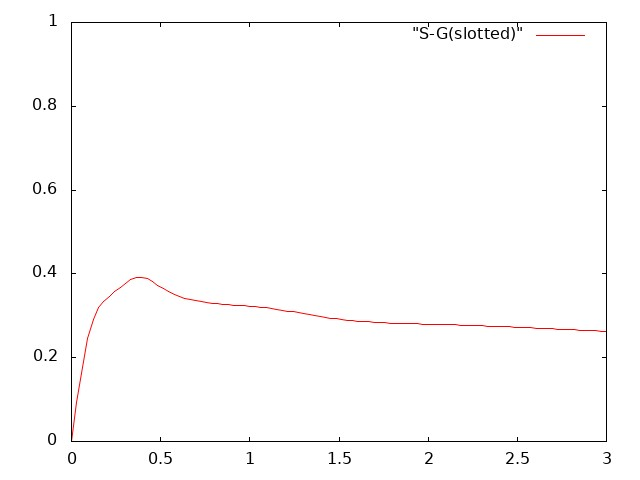
\includegraphics[width=0.5\textwidth]{2_2.jpg}
\caption{S-G Graph for Slotted ALOHA}
\end{figure}

\subsection*{Analysis}
Similarly, the results of slotted ALOHA also doesn't match well with the theory with \(S_{max} = 0.368\) at \(G = 1.0\) \\

However, fortunately, compared with data of pure ALOHA, the value of \(S\) of slotted ALOHA is always larger regardless of the value of \(G\). This phenomenon shows that slotted ALOHA has higher efficiency that pure ALOHA.



\section*{CSMA}
\subsection*{Theories}
Carrier Sense Multiple Access (CSMA) is a probabilistic Media Access Control (MAC) protocol in which a node verifies the absence of other traffic before transmitting on a shared transmission medium, such as an electrical bus, or a band of the electromagnetic spectrum. \\

"Carrier Sense" describes the fact that a transmitter uses feedback from a receiver that detects a carrier wave before trying to send. That is, it tries to detect the presence of an encoded signal from another station before attempting to transmit. If a carrier is sensed, the station waits for the transmission in progress to finish before initiating its own transmission. In other words, CSMA is based on the principle "sense before transmit" or "listen before talk". \\
"Multiple Access" describes the fact that multiple stations send and receive on the medium. Transmissions by one node are generally received by all other stations using the medium. \\

CSMA protocol has three access modes: 1-persistent, non-persistent and p-persistent.\\

1. 1-persistent \\
When the sender (station) is ready to transmit data, it checks if the transmission medium is busy. If so, it then senses the medium continually until it becomes idle, and then it transmits the message (a frame). In case of a collision, the sender waits for a random period of time and attempts to transmit again. \\

2. Non-persistent \\
Non persistent CSMA is less aggressive compared to P persistent protocol. In this protocol, before sending the data, the station senses the channel and if the channel is idle it starts transmitting the data. But if the channel is busy, the station does not continuously sense it but instead of that it waits for random amount of time and repeats the algorithm. Here the algorithm leads to better channel utilization but also results in longer delay compared to 1 -persistent. \\

3. P-persistent \\
This is a sort of trade-off between 1 and non-persistent CSMA access modes. When the sender is ready to send data, it checks continually if the medium is busy. If the medium becomes idle, the sender transmits a frame with a probability p. If the station chooses not to transmit (the probability of this event is 1-p), the sender waits until the next available time slot and transmits again with the same probability p. This process repeats until the frame is sent or some other sender starts transmitting. In the latter case the sender monitors the channel, and when idle, transmits with a probability p, and so on. p-persistent CSMA is used in CSMA/CA systems including WiFi and other packet radio systems. \\

\begin{figure}
\centering
\includegraphics[width=0.8\textwidth]{3_1.eps}
\caption{Simple Graphical Description for CSMA}
\end{figure}

\subsection*{Simulation}
The Simplified Procedure of the Program: \\

1) The program user sets the number of stations, the probability of a station having a frame to send and the duration of the program. \\
2) The program forms a new array and fills it with numbers other than 0 and 1. \\
3) The length of a frame stays a static constant the whole simulation process which is 3, i.e. \\
4) The random waiting time is set no larger than 10 and at least 3, which is the length of a frame. \\
5) The program checks to see whether the medium is idle or busy and decides which station to transmit frames. \\
(i) If the station has something to transmit and the medium is idle without ant collisions, then the station begins to send frames. \\
(ii) If the station has something to send and the medium is busy but has no collisions, it first checks whether it sent data in the last second. If true, it keeps sending. If false, it waits a random number of seconds. \\
(iii) If the station has something to send and the medium is busy and has collisions, it senses the medium continuously (per second) to send frames. \\
(iv) In all other states, the station does nothing. \\
(v) Another array with comparatively small size will be used to record the number of successively transmitted frames of each station.

\subsection*{Results}
1. For the 1-persistent CSMA case, the frame time is set to be 3 seconds. The whole process duration is 1200 seconds. The experiment data1 is in the following lists.

\begin{table}[htbp]
\begin{tabular}{lcccccccccc}
\toprule
Stations & 1 & 2 & 3 & 4 & 5 & 6 & 7 & 8 & 9 & 10 \\
\midrule
Frames & 259 & 118 & 69 & 55 & 51 & 30 & 22 & 23 & 27 & 19 \\
\bottomrule
\end{tabular}
\end{table}

\begin{table}[htbp]
\begin{tabular}{lcccccccccc}
\toprule
Stations & 11 & 12 & 13  & 14 & 15 & 16 & 17 & 18 & 19 & 20 \\
\midrule
Frames & 22 & 23 & 18 & 15 & 11 & 8 & 11 & 8 & 7 & 8 \\
\bottomrule
\end{tabular}
\end{table}

2. For the non-persistent CSMA case, the frame time is set to be 3 seconds. The whole process duration is 1200 seconds. The experiment data1 is in the following lists. 
\begin{table}[htbp]
\begin{tabular}{lcccccccccc}
\toprule
Stations & 1 & 2 & 3 & 4 & 5 & 6 & 7 & 8 & 9 & 10 \\
\midrule
Frames & 254 & 119 & 80 & 54 & 61 & 45 & 23 & 24 & 28 & 18 \\
\bottomrule
\end{tabular}
\end{table}

\begin{table}[htbp]
\begin{tabular}{lcccccccccc}
\toprule
Stations & 11 & 12 & 13  & 14 & 15 & 16 & 17 & 18 & 19 & 20 \\
\midrule
Frames & 22 & 13 & 13 & 6 & 12 & 8 & 8 & 2 & 6 & 5 \\
\bottomrule
\end{tabular}
\end{table}

3. For the p-persistent CSMA case, the frame time is set to be 3 seconds. The whole process duration is 1200 seconds, and the number of users is 10. The experiment data1 is in the following lists.
\begin{table}[htbp]
\begin{tabular}{lccccccccccc}
\toprule
p & 0.05 & 0.10 & 0.15  & 0.20 & 0.25 & 0.30 & 0.35 & 0.40 & 0.45 & 0.50 \\
\midrule
Frames & 37 & 52 & 76 & 80 & 99 & 98 & 113 & 129 & 142 & 144 \\
\bottomrule
\end{tabular}
\end{table}

\begin{table}[htbp]
\begin{tabular}{lccccccccccc}
\toprule
p & 0.55 & 0.60 & 0.65  & 0.70 & 0.75 & 0.80 & 0.85 & 0.90 & 0.95 & 1.00 \\
\midrule
Frames & 158 & 155 & 152 & 162 & 178 & 195 & 199 & 200 & 205 & 202 \\
\bottomrule
\end{tabular}
\end{table}

\subsection*{Analysis}


\section*{CSMA/CD}
\subsection*{Theories}
At a given moment, user A has a packet to send. Before starting transmission, it checks whether the medium is idle or not. If the medium is busy, the user waits a random time and then tries again. If the medium is idle, the user starts to transmit, and keeps sensing the medium. Once a collision signal is detected, rather than finishing sending the packet, the station stops sending immediately and waits for the next attempt. \\

For choosing the random time, the protocol uses the Binary Exponential Backoff Algorithm. According to the algorithm, time is divided into discrete slots whose length is equal to the worst-case round-trip propagation time on the ether. After the first collision, the station waits either 0 or 1 slot time before another try. After the second collision, the station chooses either 0, 1, 2 or 3 slots randomly and waits that number of slot time. Thus, by the same rule, after kth collision, the number of time slots to wait is chosen randomly from the interval 0 to \(2^k-1\). \\

Theoretically, the maximum throughput is given by: \\

\qquad \(\rho_{max} = \frac{X}{X+t_{prop}+2et_{prop}} = \frac{1}{1+(2e+1)a}\) \\
where \(a = \frac{t_{prop}}{X} = \frac{Rd}{vL}\) \\
(\(R\): transmission rate, \(L\): frame length, \(v\): light speed in medium, \(d\): diameter of system, \(X\): frame time).

\subsection*{Assumptions}
1. The propagation time is assumed to be the smallest time unit in the entire design and set to be 1 time slot. \\
2. The "medium" is set to be a station with 1 time slot delay to all other stations. \\
3. The duration of the simulation is in the unit of time slots. \\
4. The states of all users during the whole process are saved in a large array and the size of it is the number of users times the duration.

\subsection*{Simulation}
The Flow Chart of the Program is shown on "Figure 6". \\
\begin{figure}
\centering
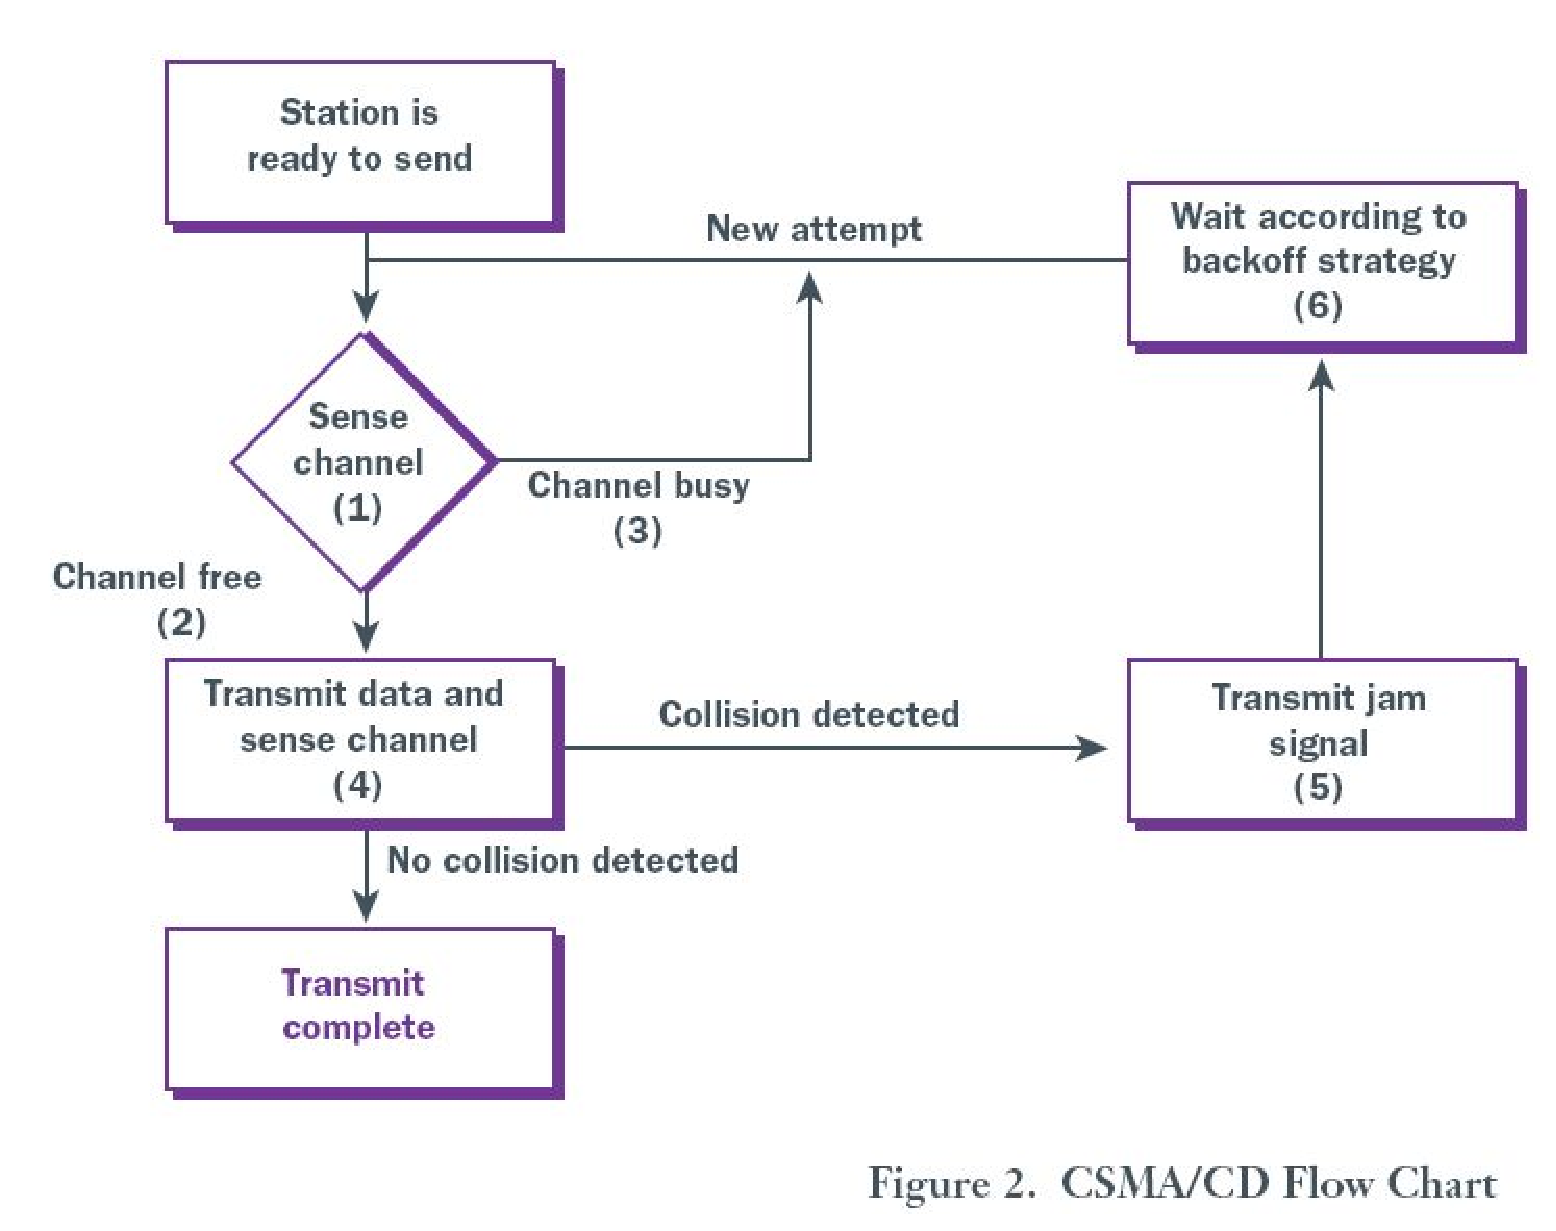
\includegraphics[width=0.7\textwidth]{4_1.eps}
\caption{Flow Chart for CSMA/CD Simulation}
\end{figure}

The Simplified Procedure of the Program: \\

1) The program user sets the number of stations, the probability of a station having a frame to send and the duration of the program. \\
2) The program forms a new array and fills it with numbers other than 0 and 1. \\
3) Using the function "setFrame()" to make the array initialized with 0s and 1s. If the frame time is set to be 4, then every 4 consecutive 1s at a position of the array means a certain station at that time will have a frame to send. \\
4) The program set a "for" loop that repeats the value of duration times. In each loop, it contains another "for" loop, which repeats the number of stations times. In each small loop, the program checks the state of one station. \\
(i) If the station has something to send and the medium is idle, then the station begins to send and the data it is sending will be received by the medium in the next larger loop. \\
(ii) If the station has something to send and the medium is busy but has no collisions, it first checks whether it sent data in the last two loops. If true, it keeps sending. If false, it waits a random number of slots based on the Binary Exponential Backoff Algorithm. The act “Waiting” is realized by postponing the value in the array by a given slots. Values, which are moved out of bound, are just discarded and the newly - produced empty slots are filled by 0s. \\
(iii) If the station has something to send and the medium is busy and has collisions, it does the same backoff strategy as in the previous part. \\
(iv) In all other states, the station does nothing. \\
(v) After each small loop, the program checks the state of the medium and report the change by changing values of several parameters. These parameters will be checked at the first of next large loop in order to simulate the one-slot delay. \\
(vi) Another array with comparatively small size will be used to record the number of successively transmitted frames of each station.

\subsection*{Results}
1. For the original case, the frame time is set to be 4 slots. The whole process duration is 1000 slots, and the number of users is 10. The experiment data1 is in the following lists and the graph is shown on "Figure 7". (Since the theoretical values are measured without using BEBA, so in this case, all stations wait a random time from 0 to 1024 slots) \\
\begin{table}[htbp]
\begin{tabular}{lccccccccccc}
\toprule
p & 0.05 & 0.10 & 0.15  & 0.20 & 0.25 & 0.30 & 0.35 & 0.40 & 0.45 & 0.50 \\
\midrule
Num & 36 & 37 & 35 & 34 & 33 & 30 & 29 & 27 & 25 & 25 \\
\bottomrule
\end{tabular}
\end{table}

\begin{table}[htbp]
\begin{tabular}{lccccccccccc}
\toprule
p & 0.55 & 0.60 & 0.65  & 0.70 & 0.75 & 0.80 & 0.85 & 0.90 & 0.95 & 1.00 \\
\midrule
Num & 22 & 22 & 20 & 20 & 18 & 17 & 16 & 15 & 14 & 13 \\
\bottomrule
\end{tabular}
\end{table}

\begin{figure}
\centering
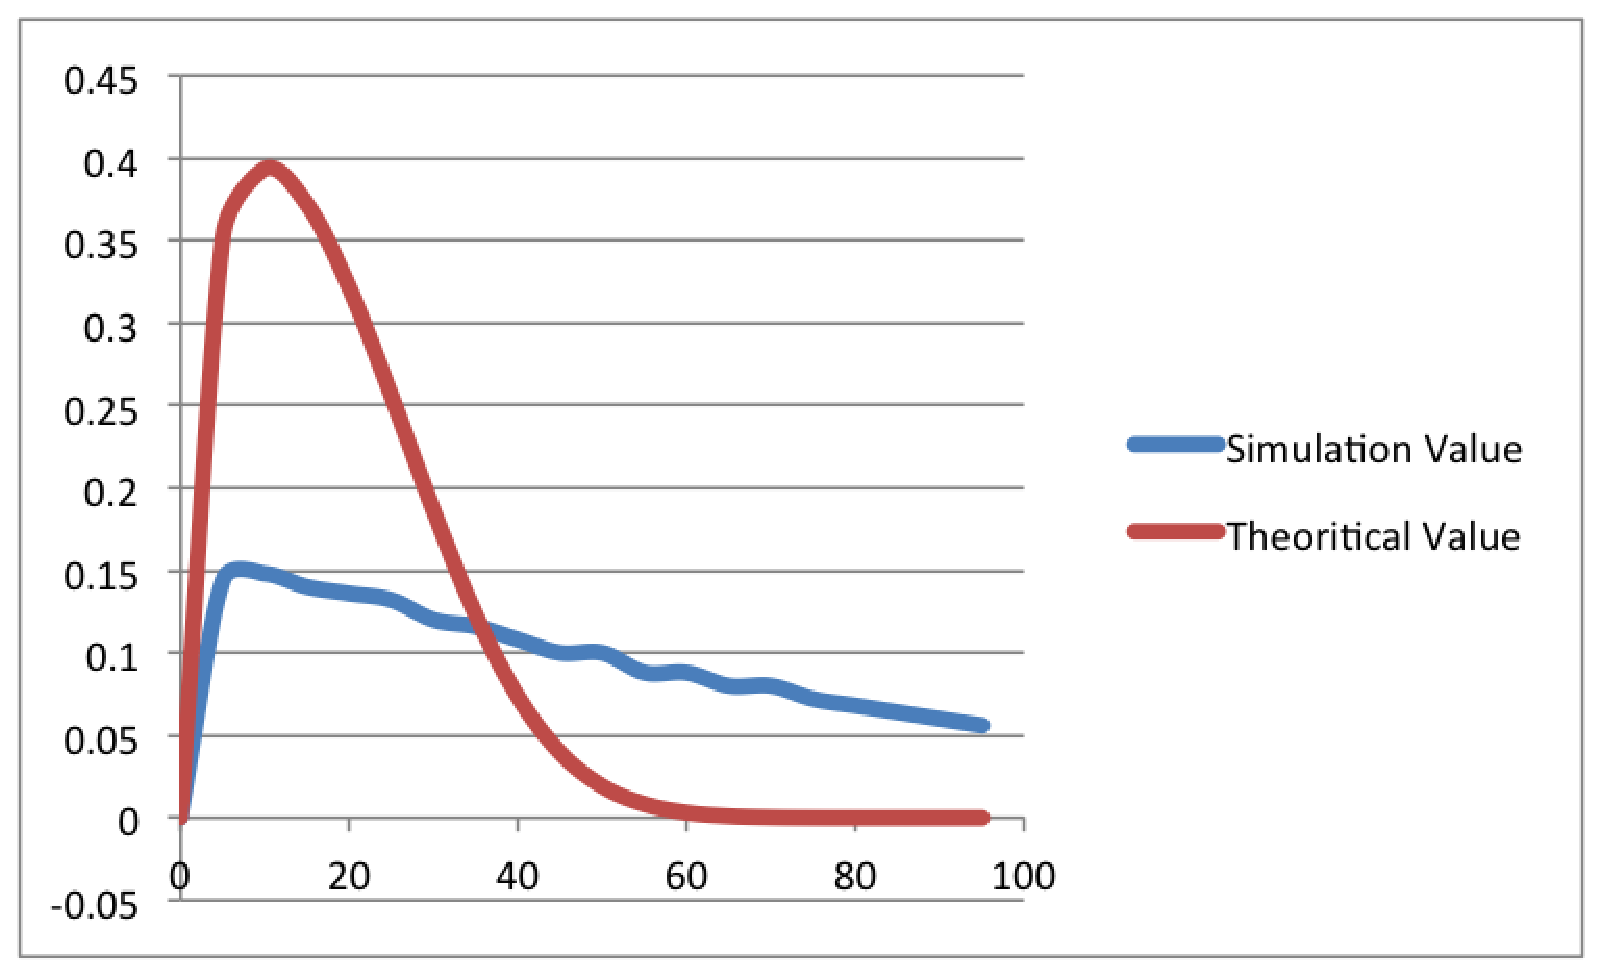
\includegraphics[width=0.6\textwidth]{4_2.eps}
\caption{n-p Graph for Sample 1}
\end{figure}

2. To show the influence of BEBA, the program simulates the same situation as in the first case both with BEBA and without it. The data of the one with BEBA is shown in the following list. \\
\begin{table}[htbp]
\begin{tabular}{lccccccccccc}
\toprule
p & 0.05 & 0.10 & 0.15  & 0.20 & 0.25 & 0.30 & 0.35 & 0.40 & 0.45 & 0.50 \\
\midrule
Num & 55 & 56 & 57 & 59 & 63 & 63 & 67 & 69 & 73 & 76 \\
\bottomrule
\end{tabular}
\end{table}

\begin{table}[htbp]
\begin{tabular}{lccccccccccc}
\toprule
p & 0.55 & 0.60 & 0.65  & 0.70 & 0.75 & 0.80 & 0.85 & 0.90 & 0.95 & 1.00 \\
\midrule
Num & 82 & 86 & 93 & 98 & 104 & 111 & 114 & 118 & 119 & 119 \\
\bottomrule
\end{tabular}
\end{table}

The figure of the performance of this situation is shown in "Figure 8", comparing to the performance of the one without Binary Exponential Backoff Algorithm.
\begin{figure}
\centering
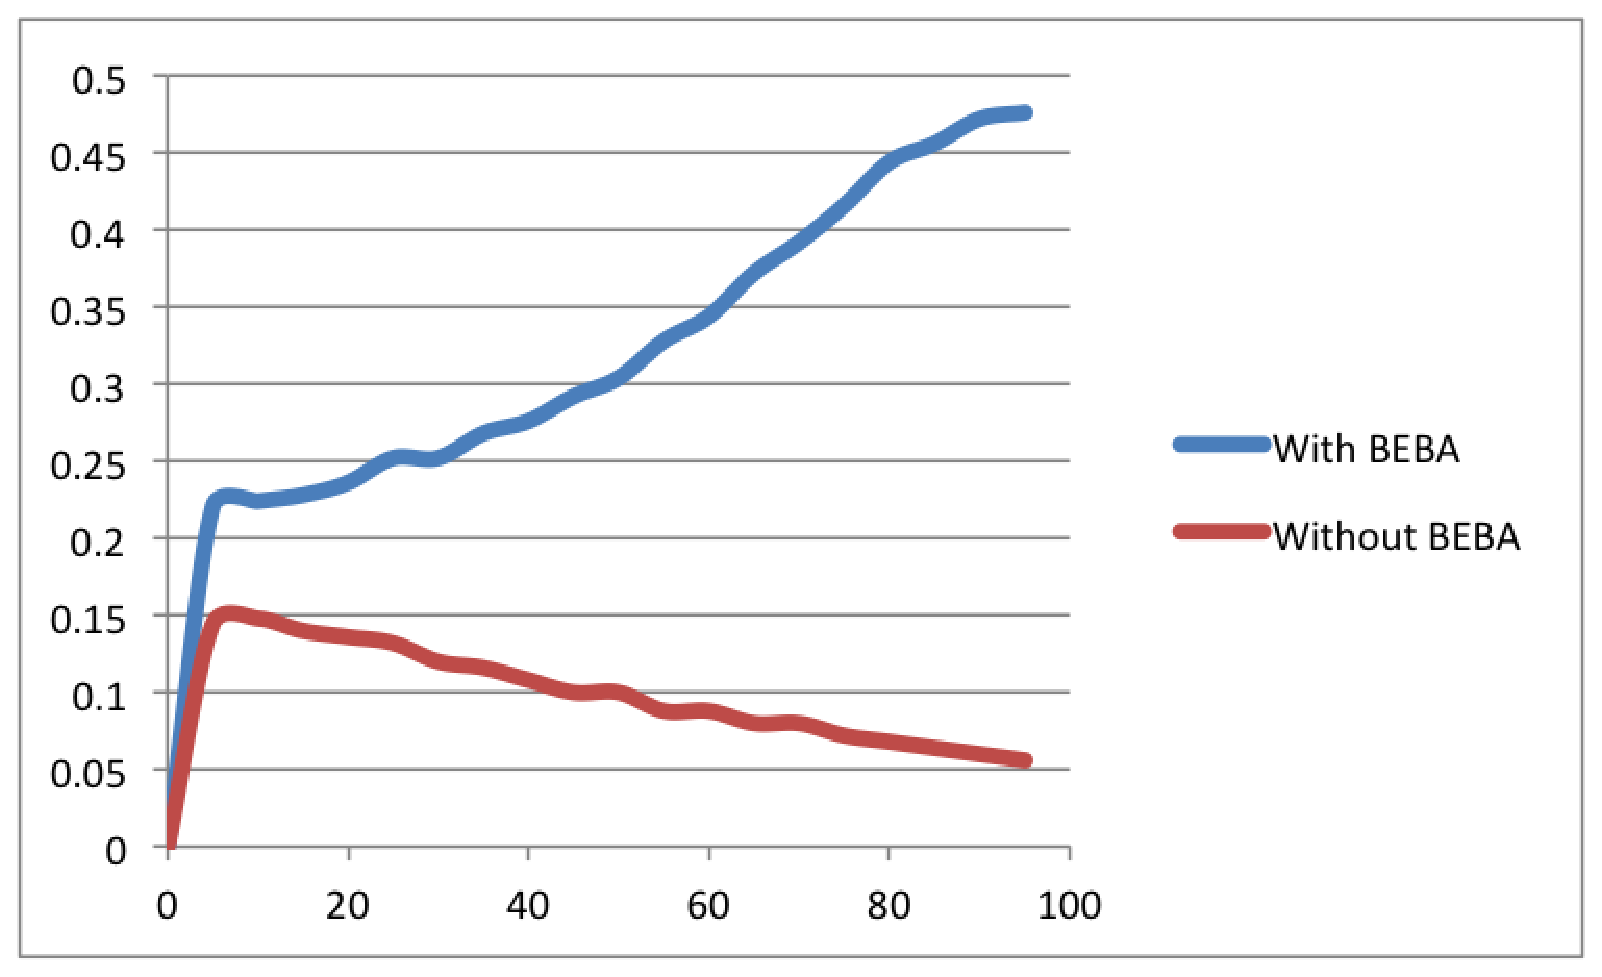
\includegraphics[width=0.6\textwidth]{4_3.eps}
\caption{n-p Graph for Sample 2}
\end{figure}

3. In order to find out the relationship between performance and number of users, the first case is tested again by changing the number of users to be 5. The experiment data is in the following lists. \\
\begin{table}[htbp]
\begin{tabular}{lccccccccccc}
\toprule
p & 0.05 & 0.10 & 0.15  & 0.20 & 0.25 & 0.30 & 0.35 & 0.40 & 0.45 & 0.50 \\
\midrule
Num & 25 & 28 & 27 & 26 & 21 & 21 & 18 & 18 & 16 & 14 \\
\bottomrule
\end{tabular}
\end{table}

\begin{table}[htbp]
\begin{tabular}{lccccccccccc}
\toprule
p & 0.55 & 0.60 & 0.65  & 0.70 & 0.75 & 0.80 & 0.85 & 0.90 & 0.95 & 1.00 \\
\midrule
Num & 14 & 11 & 11 & 10 & 10 & 9 & 9 & 8 & 8 & 8 \\
\bottomrule
\end{tabular}
\end{table}

The figure of the performance of this situation is shown in "Figure 9", comparing to the performance of the one with ten users.
\begin{figure}
\centering
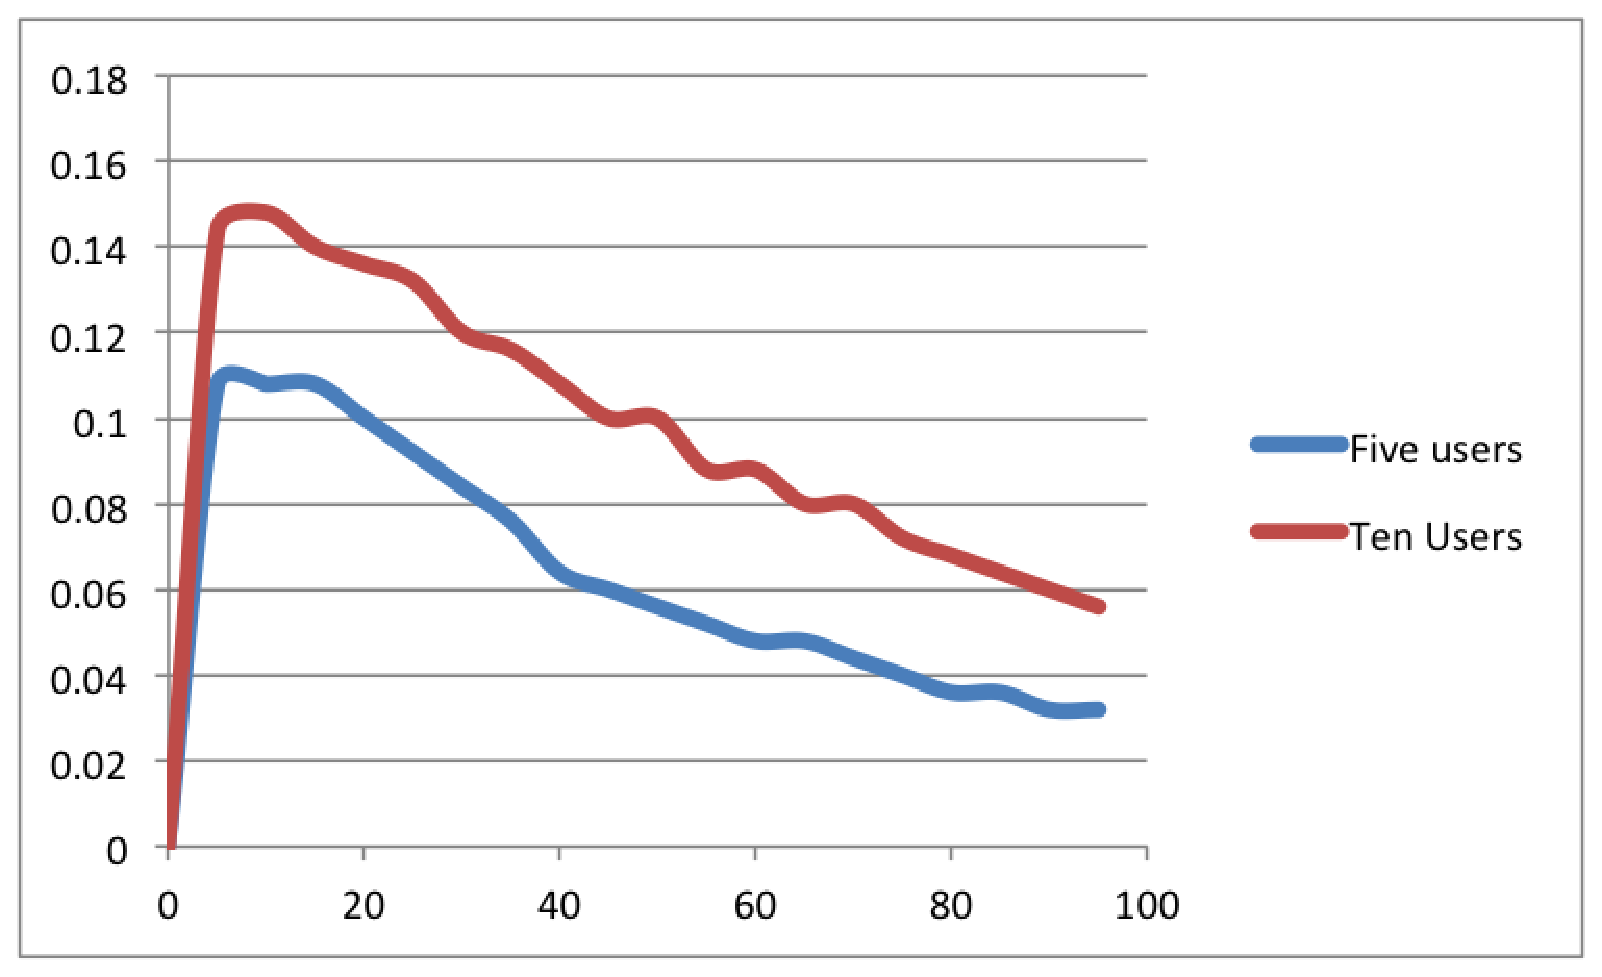
\includegraphics[width=0.6\textwidth]{4_4.eps}
\caption{n-p Graph for Sample 3}
\end{figure}

4. To see the efficiency change due to the ratio of propagation time and frame time, a new simulation is done with the set used in the first one except that the frame time is set to be 10. The whole process is 1000. The experiment data is in the following lists.
\begin{table}[htbp]
\begin{tabular}{lccccccccccc}
\toprule
p & 0.05 & 0.10 & 0.15  & 0.20 & 0.25 & 0.30 & 0.35 & 0.40 & 0.45 & 0.50 \\
\midrule
Num & 21 & 23 & 24 & 24 & 24 & 22 & 21 & 21 & 19 & 20 \\
\bottomrule
\end{tabular}
\end{table}

\begin{table}[htbp]
\begin{tabular}{lccccccccccc}
\toprule
p & 0.55 & 0.60 & 0.65  & 0.70 & 0.75 & 0.80 & 0.85 & 0.90 & 0.95 & 1.00 \\
\midrule
Num & 18 & 18 & 17 & 16 & 15 & 15 & 14 & 14 & 13 & 13 \\
\bottomrule
\end{tabular}
\end{table}

The figure of the performance of this situation is shown in "Figure 10", including the theoretic value at this situation.
\begin{figure}
\centering
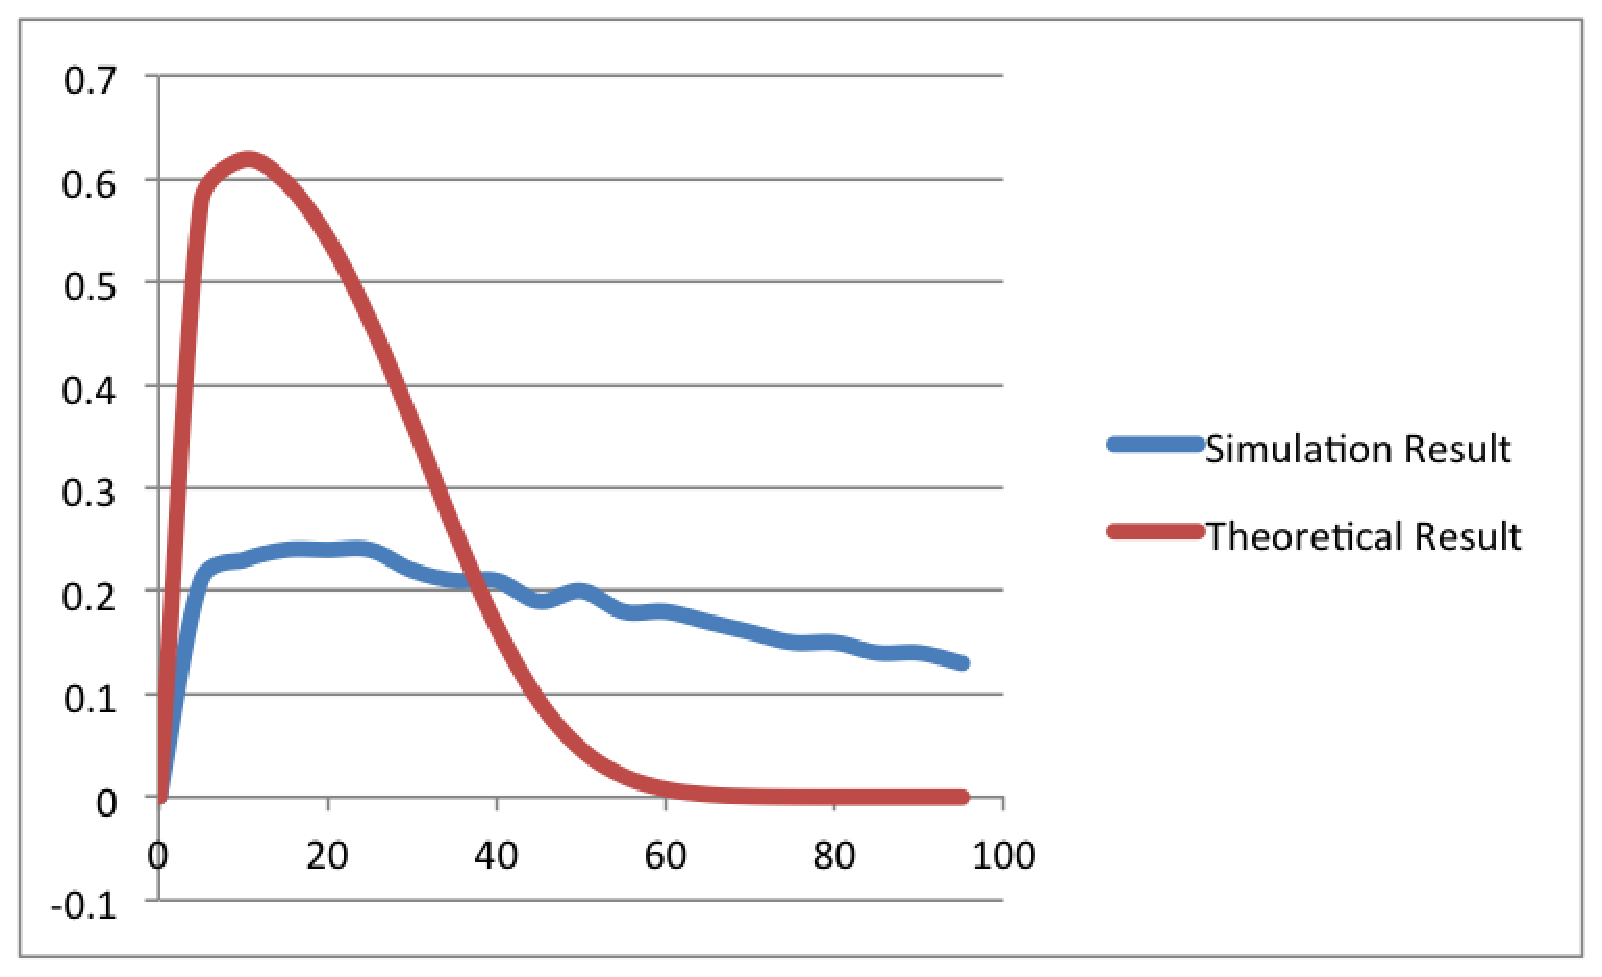
\includegraphics[width=0.6\textwidth]{4_5.eps}
\caption{n-p Graph for Sample 4}
\end{figure}

\subsection*{Analysis}
From the figures of Sample 1 and Sample 4, which show the difference between experimental and theoretical results, it can be inferred by both curves that the highest transmission efficiency happens when \(n = 1/p\), and \(G = 1\). However, there are some obvious errors between two results. One of them is that the simulation cannot reach as high efficiency as in theory. The most important reason may be that in the process of calculating the theoretical result, it doesn’t take the influence of random waiting time into account because the theoretical result is just based on the probability of just one attempt per frame time. So with different scope of random waiting slots, the result may differ a lot. \\ 

Another big difference is that according to the theory, the efficiency at the point \(p = 1\) should be zero. But in the simulation, the value is a positive integer. It is quite reasonable to see that because since the number of slots ranges from 0 to a number larger than half of the entire duration. If some of stations just wait a few slots while others wait much more time, then these stations would have enough time to finish their transmission. But this kind of transmission will cause a very large delay, which means that it is not suitable for many heavy-traffic users. \\

Between the two figures, we can see that the one with smaller \(A\) (propagation time divided by frame time) has better performance, which is the same as illustrated in the textbook. \\

In the second simulation, which compares the program both with and without BEBA. From the figure, it is clear that the one with BEBA performs much better than the one without BEBA. And instead of having bad performance, the one with BEBA has a better efficiency when p increases. Thus as a conclusion of the result of simulation, it is better to choose BEBA as the algorithm of setting random waiting time when the traffic is very heavy. \\

For the third simulation, it tells that when user numbers are larger, the performance will be better. This result is expected because when calculating the maximum efficiency, an approximation is made at \((1-\frac{1}{n})^{n-1}\) when \(n\) is large enough. However, one problem emerges. In the theory, the probability of a transmission success is \(P_s = np(1-p)^{n-1}\), and the maximum value happens when \(n = \frac{1}{p}\). Thus the peak value of \(S\) should happens at \(p = \frac{1}{n}\), but in the figure, the two peak values of different curves happen at the same point. This error may be caused by the scale of simulation or some little errors in the design of simulation. \\

Comparing to ALOHA and Slotted ALOHA, CSMA has greatly improved the efficiency of transmission. However, a user who is sending a frame needs time, which is twice of the propagation time, to capture the medium. During this small time interval, other users who happen to have packets to send may regard the medium as idle and begins to transit and thus destroys both packets. And with the increasing of propagation time caused by longer distance or lower transmission rate, this kind of fault will have larger effect and reduces the efficiency rapidly. \\

In order to minimize the influence of problem mentioned above, CSMA/CD (collision detection) is invented. It tells users whether their packets are having collisions with other packets or not. If true, both the users stop transmission to save time and wait for another chance.
\end{document}


